\section{Allgemeines}

Obwohl Rice das ASP schon 1976 vorstellte und die Formalisierung des Ökonomieportfolios mehr als 50 Jahre alt ist, wurde die Idee der Algorithmenportfolios erst im Zusammenhang mit Restartstrategien 1997 das erste Mal betrachtet \cite{huberman97}. Durch Restartstrategien werden Algorithmen neugestartet, sobald bestimmte Kriterien erfüllt sind (siehe Abschnitt \ref{restartstrategien}).

Algorithmenportfolios bieten Möglichkeiten mit den Schwierigkeiten des ASP umzugehen. Grundlegender Gedanke dabei ist es nicht nur einen einzelnen Algorithmus für die Berechnung von Probleminstanzen auszuwählen, sondern eine Untermenge der verfügbaren Algorithmen. Wichtig ist zu erwähnen, dass ein Algorithmus mehrmals in einem Portfolio vorkommen kann. Die ausgewählten Algorithmen sollen dann für möglichst viele Problemklassen gute Leistungen erzielen und eine kleine Varianz in der Laufzeit zwischen Probleminstanzen des gleichen Typs liefern. 

Beide Kriterien, Laufzeit und Varianz, sind ähnlich den beiden Kriterien der Ökonomie"-portfolios, erwartetem Gewinn und Varianz dessen. Jedoch gibt es auch gravierende Unterschiede, weshalb sich die Anwendung der Theorie der Portfolios aus der Ökonomie auf die Algorithmenportfolios teilweise schwierig gestaltet \cite{gomesselman97}. Zur Verdeutlichung seien an dieser Stelle zwei Schwierigkeiten erwähnt. Zum einen muss man sich bei Algorithmenportfolios eine Ausführungsart der Algorithmen überlegen, obgleich sich der Markt in der Wirtschaft ohne eigenes Zutun weiterentwickelt. Und zum anderen summieren sich Gewinne und Verluste von Anlagen eines Portfolios, während mehrere Algorithmen mit guten Laufzeiten für die gleiche Probleminstanz keinen Mehrwert gegenüber einem einzigen guten Algorithmus im Portfolio für diese Probleminstanz haben.

Ein Problem bei der allgemeinen Betrachtung von Algorithmenportfolios anhand der vorhandenen Forschung ist vielfach die Spezialisierung der Analysen auf einzelne Problemtypen, welche meist Entscheidungs- oder Optimierungsprobleme sind. So wird beispielsweise in \cite{fukunaga99} das \textit{Traveling Salesman Problem} (TSP) zur Evaluierung herangezogen, das \textit{Mixed Integer Problem} (MIP) in \cite{gomesselman97} und oft das \textit{Erfüllbarkeitsproblem} (SAT) wie zum Beispiel in \cite{kautz02}. Aus diesem Grund müssen viele Ansätze und Methoden kritisch betrachtet werden, da sie keiner allgemeineren Evaluierung unterzogen wurden.

\subsection{Restartstrategien}
\label{restartstrategien}

Stochastische Algorithmen können mit verschiedenen Parametern und Startwerten für Zufallszahlengeneratoren unterschiedliche Leistungen erbringen. Eine Ursache dafür kann sein, dass ein Algorithmus für die Berechnung der Lösung eines Problems den Suchraum stochas"-tisch verkleinert. Ist eine Lösung innerhalb dieses kleineren Suchraums kann sie nun schneller gefunden werden. Ist keine Lösung im verkleinerten Suchraum sind die Berechnungen für diesen Suchraum überflüssig. Werden wiederholt Suchräume ohne Lösung ausgewählt verlängert sich dementsprechend die Laufzeit. Variiert die Leistung des Algorithmus stark, seien solche Algorithmen an dieser Stelle als riskant, ansonsten als sicher bezeichnet. Riskante Algorithmen haben den Vorteil bei guten Läufen meistens wesentlich bessere Ergebnisse zu erzielen als sichere Algorithmen. Belegt ein SAT Algorithmus beispielsweise einige Formelvariablen zufällig mit Werten und es stellen sich diese als Werte einer potentiellen Lösung dar, wird der Suchraum, wie oben beschrieben, verkleinert und es kann schneller eine Lösung gefunden werden. Führen die zufälligen Belegungen jedoch zu keiner Lösung hat dieser Teil der Suche nur unnötige Kosten verursacht. Um solche Verfahren zu systematisieren werden beispielsweise Heuristiken eingesetzt \cite{brelaz79, gomesselman97}.

Ursprünglich wurden Restartstrategien verwendet um Algorithmen, welche bei lokalen Maxima festhingen, davon loszulösen \cite{kautz02}. Mittlerweile verfolgen Restartstrategien haupt"-sächlich das Ziel stochastische Algorithmen neuzustarten, sobald sich erkennen lässt, dass ein ungünstiger Lauf durchgeführt wird. Besonders effektiv ist diese Methode bei 'heavy-tailed' Laufzeitverteilungen (siehe Abbildung \ref{heavytailed}). Die Annahme dahinter ist, dass die Wahrscheinlichkeit mit der ein stochastischer Algorithmus eine Lösung zum aktuellen Zeitpunkt findet mit zunehmender Laufzeit sinkt, sodass ein Neustart ab einem bestimmten Zeitpunkt effektiver ist. \\

\begin{figure}[h]
\centering
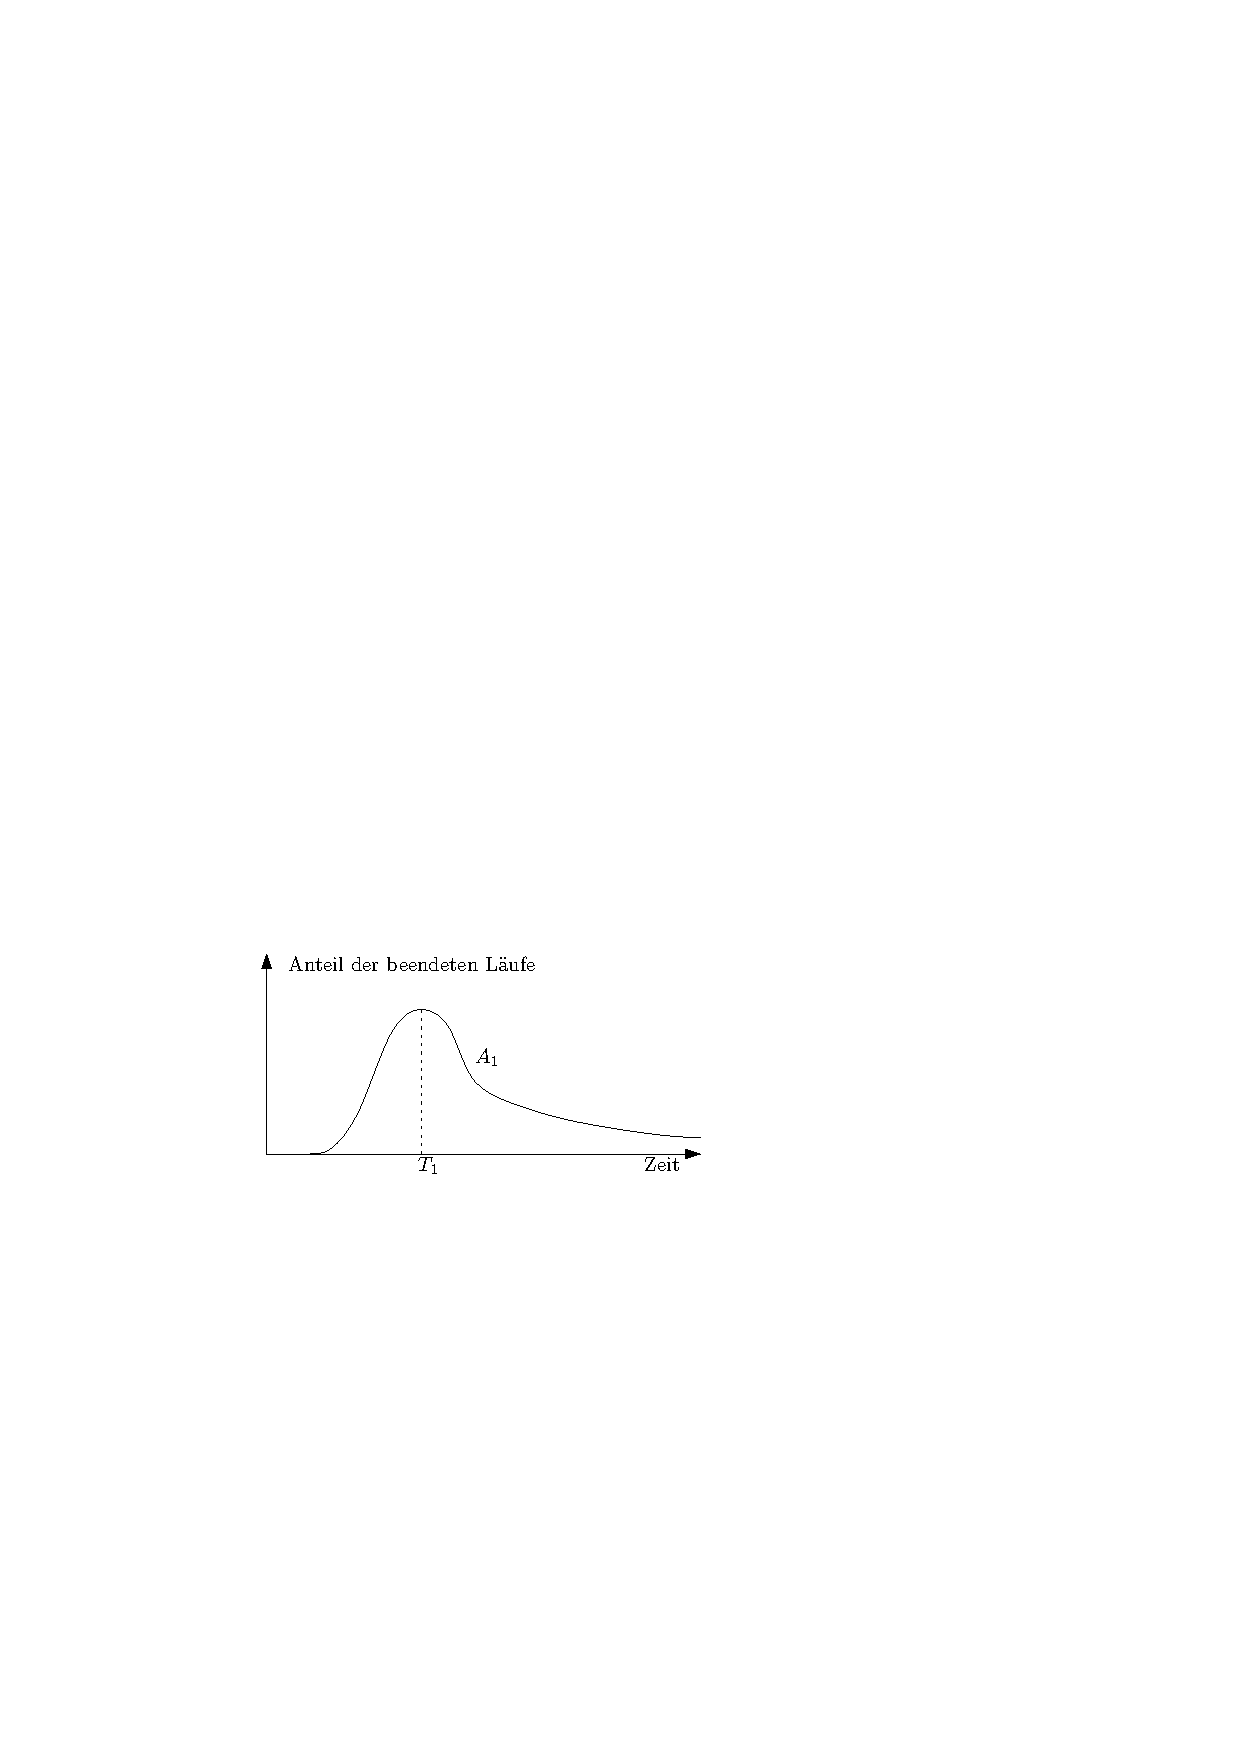
\includegraphics{heavytailed.pdf}
\caption[Heavy-Tailed Laufzeitverteilung]{Zum Zeitpunkt $T_1$ terminieren die meisten Läufe des Algorithmus $A_1$. Mit zunehmender Zeit nimmt diese Anzahl nur langsam ab, sodass einige Ausführungen eine sehr lange Laufzeit haben. Für solch eine Ausführung ist ein Neustart oft effektiver als den Algorithmus terminieren zu lassen.}
\label{heavytailed}
\end{figure}

Der optimale Zeitpunkt für den Neustart zur Minimierung der erwarteten Laufzeit kann berechnet werden, sofern komplettes Wissen über die Laufzeitverteilung vorhanden und die Laufzeit das einzige Kriterium zur Bewertung des Algorithmus ist \cite{kautz02}. Im Allgemeinen ist dieses Wissen nicht verfügbar. Daher gibt es einige Methoden um dieses Problem zu umgehen. Eine Möglichkeit ist es eine Trainingsphase durchzuführen, in der verschiedene Zeiten und verschiedene Probleme benutzt werden um einen guten Zeitpunkt zu berechnen. Der gefundene Zeitpunkt kann dann durch dynamisches Anpassen zwischen Problemberechnungen oder direkt nach einem Neustart weiter verbessert werden. Diese Anpassung ist bei einer Trainingsphase mit wenigen Problemlösungen sehr effektiv.\footnote{In \cite{gaglioloschmidhuber07} werden bis zu sechs mal bessere Ergebnisse mit zusätzlicher Anpassung des Zeitpunkts erzielt.} Sie ermöglicht jedoch keine prinzipiell besseren Ergebnisse als eine Trainingsphase mit vielen Problemlösungen \cite{fukunaga99}. 

Eine interessante Erkenntnis dieser Lernmethoden ist, dass sogar bessere Ergebnisse als mit dem optimalen Zeitpunkt erzielt werden können \cite{kautz02}. Das hängt damit zusammen, dass der optimale Zeitpunkt mathematisch mithilfe der Wahrscheinlichkeitsverteilung für die Terminierung eines Algorithmus berechnet wird. Diese Verteilung tritt bei einer konkreten Durchführung natürlich nicht genau in dieser Form auf, sodass der optimale Zeitpunkt für einen konkreten Fall nicht mit dem allgemeinen optimalen Zeitpunkt übereinstimmen muss.

Die Idee der Restartstrategien kann auch auf Algorithmenportfolios übertragen werden. Wichtig dabei ist, dass ein Algorithmus mehrmals in einem Portfolio vorkommen kann. Dieser wird dann bei der Durchführung parallel mit unterschiedlichen Parametern und/oder Anfangswerten für Zufallszahlengeneratoren ausgeführt. Folglich kann im Extremfall ein Algorithmenportfolio nur aus einem Algorithmus bestehen. In \cite{gomesselman97} wird dieses Szenario genauer analysiert. Es werden 2 Algorithmen, einer davon riskant und einer sicher, zur Lösung des MIP als Kandidaten für ein Algorithmenportfolio betrachtet. Zudem werden vier Größen (2, 5, 10, 20) des Portfolios untersucht. Das Ergebnis dieser Arbeit ist folgendes: Je mehr Algorithmen im Portfolio vorhanden sind, desto besser ist es wenn nur der riskante Algorithmus mehrfach vorhanden ist. Die Erklärung ist naheliegend. Wird der riskante Algorithmus öfter ausgeführt steigt die Wahrscheinlichkeit einen guten Lauf unter den Ausführungen zu erhalten.

Im Zusammenhang mit Simulationsproblemen sind Restartstrategien nur bedingt sinnvoll einsetzbar. Zum einen haben Simulationsalgorithmen nicht immer eine 'heavy-tailed' Laufzeitverteilung. Zum anderen müssen sie auch nicht stochastisch sein, sodass ein Neustart nur gleiche neue Berechnungen verursachen würde. Auf Grund dessen muss über den Einsatz von Restartstrategien im Einzelfall entschieden werden. Darüber hinaus muss folgendes Szenario bedacht werden: Benötigt ein Lauf eines Simulationsalgorithmus viel Laufzeit, kann es daran liegen, dass dieser einen unwahrscheinlichen und aufwändigen Verlauf des Modells berechnet. Ein Neustart würde diesen Verlauf dann aus den beobachteten Durchläufen löschen. Das würde bedeuten, dass am Ende der Simulation kein aufwändiger Verlauf berechnet wurde und die Endergebnisse verfälscht und unbrauchbar sind.

\subsection{Auswahl der Algorithmen}

Das Auswahlverfahren der Algorithmen für ein Portfolio ist oft nicht näher erläutert oder dem Benutzer überlassen. In dem viel referenzierten Werk von Schmidhuber und Gagliolo \cite{gaglioloschmidhuber06} heißt es: "`At the lowest level, the choice of the algorithms composing $\mathcal{A}$ [...] is still left to the user"'. In \cite{fukunaga99} wird ein einfacher Algorithmus zur Konstruktion von Portfolios angegeben. Dieser benötigt jedoch eine große Datenbasis um zweckmäßige Ergebnisse zu liefern und kann nur bei Portfolios angewendet werden die eine konstante Laufzeit $T$ haben. In der Datenbasis werden die einzelnen Leistungen der Algorithmen nach $T$ Zeiteinheiten für eine gewisse Anzahl an Problemen gespeichert und zur Berechnung des nach diesen Daten optimalen Portfolios genutzt. In Folge dessen ist das gefundene Portfolio letztendlich für die bereits gelösten Probleme optimal, jedoch nicht zwangsweise für weitere Probleme. Beide Kriterien für diesen Konstruktionsalgorithmus werden im Allgemeinen nicht erfüllt.

Des Weiteren ist die Anzahl der Algorithmen in den betrachteten Portfolios meistens kleiner als 10 \cite{fukunaga99, gomesselman97}. Ob sich gute Ergebnisse auch mit einer großen Anzahl von Algorithmen erzielen lassen bleibt unklar.

Im Zusammenhang mit Restartstrategien haben Gomes und Saleman \cite{gomesselman97} gezeigt, dass es im Allgemeinen besser ist Algorithmen in das Portfolio aufzunehmen, welche für wenige Probleme sehr gute Ergebnisse statt für viele Probleme durchschnittliche Ergebnisse erzielen.

Letztendlich ist aus den genannten offenen Fragen auch im Zusammenhang mit Simulationsproblemen noch Forschung notwendig um herauszufinden, wie gute Portfolios konstruiert werden sollten. Die zuletzt genannte Annahme von Gomes und Saleman sollte sich auch auf Simulationsalgorithmen übertragen lassen. Auf zelluläre Automaten übertragen, würde man solche Algorithmen nehmen, welche in bestimmten Situationen sehr gute Leistungen erbringen. Ist das Feld eines deterministischen zellulären Automaten beispielsweise hauptsächlich homogen und wenig Zellen ändern ihren Zustand bei einer Zustands"-über"-führung, wären Algorithmen im Vorteil, welche die sich nicht ändernden Flächen als solche erkennen und für entsprechende Zustandsüberführungen nicht weiter betrachten. Wechseln dagegen viele Zellen ihren Zustand ist womöglich ein Algorithmus besser, welcher immer das gesamte Feld betrachtet. Solche speziellen Algorithmen sind, sofern sie ihre Struktur optimal einsetzen können, allgemeineren Algorithmen überlegen. Folglich sollte ein Portfolio die spezielleren Algorithmen enthalten, wenn mindestens ein Algorithmus für jede Situation sehr gute Leistung erbringen wird.

\subsection{Problemtypen und Leistungsbewertung}

Zwei grundlegende Problemtypen werden bei den meisten Arbeiten unterschieden: Ent"-scheidungs- und Optimierungsprobleme \cite{gaglioloschmidhuber06, gomesselman97}. Des Weiteren wird davon ausgegangen, dass alle Algorithmen terminieren. Während nun Algorithmen für Entscheidungsprobleme ein eindeutiges Ende besitzen, sobald sie eine Lösung gefunden oder die Unlösbarkeit des Problems bewiesen haben, ist es bei Optimierungsproblemen nicht so eindeutig. Man muss sich überlegen nach welchen Kriterien man die Berechnung abbrechen möchte. Entweder ab dem Zeitpunkt zu dem eine an dem Optimum genügend dicht liegende Lösung gefunden wurde oder nach einer bestimmten Zeit oder beides (siehe Abbildung \ref{optimizationproblem}). Je nach Entscheidung muss sich das Portfolio anpassen. Wenn man die Berechnung beispielsweise durch eine Zeit begrenzt, dann müssen die Algorithmen in dieser Zeit so gut wie möglich vorankommen. Dann ist es irrelevant, ob ein Algorithmus zu einem späteren Zeitpunkt wesentlich bessere Ergebnisse als alle anderen liefern würde. Setzt man dagegen ein Qualitätsminimum könnte genau dieser Algorithmus der einzige sein, welcher dieses Minimum je erreicht.

In der Simulation treten beide Problemtypen in dieser standardisierten Form nicht auf. Beispielsweise die Zustandsüberführung eines zellulären Automaten ist weder ein Ent"-schei"-dungs- noch ein Optimierungsproblem. Nichtsdestotrotz kann man die beiden Kriterien der Laufzeit und Qualität einer Berechnung auch für Simulationsprobleme nutzen. Jedoch ist eine einfache Übernahme der theoretischen Erkenntnisse über Entscheidungs- und Optimierungsprobleme im Zusammenhang mit Algorithmenportfolios nicht möglich. 

Ein weiterer wichtiger Bestandteil bei der Arbeit mit Algorithmenportfolios ist die Bewertung ihrer Leistung. In \cite{gomesselman97} wird ein Kompromiss zwischen erwarteter Laufzeit und dessen Varianz zur Lösung eines Problems als Maßstab herangezogen. Bei Optimierungsproblemen kann zusätzlich noch die Qualität der Lösungen eine Rolle spielen. Ein weiteres Kriterium kann die Vorhersagegenauigkeit des Portfolios sein. Damit ist gemeint, ob die vorhandenen Ressourcen auch zum größten Teil dem besten Algorithmus zur Verfügung gestellt werden. Probleme bereiten dynamische Portfolios, die ihre Leistung mit zunehmender Anzahl an gelösten Problemen verbessern und daher von Beginn an unter Berücksichtigung ihres Potentials anders bewertet werden müssen (siehe Abschnitt \ref{dynamisch}).

Neben den bisher genannten Kriterien der Laufzeit und Qualität müssen bezüglich der Laufzeit bei Simulationsalgorithmen weitere Sachverhalte beachtet werden. Man sollte zur Bewertung eines Portfolios nicht nur die physische Laufzeit, sondern auch Simulationszeit heranziehen. Muss ein Algorithmus beispielsweise mehr Events als ein anderer in derselben Simulationszeit ausführen, wäre ein direkter Vergleich der physikalischen Zeit ungerecht. In Folge dessen muss auch die Anzahl der ausgeführten Events mit berücksichtigt werden. Nicht zu vergessen mögliche unterschiedliche Berechnungsaufwände von Events. Bei zellulären Automaten zum Beispiel wäre eine Zustandsüberführung eines beinahe homogenen Feldes, bei dem sich nur einige Zellen ändern einfacher zu berechnen als die Zustandsüberführung eines Feldes, bei dem sich fast alle Zellen ändern. Eine analoge Situation wie in Abbildung \ref{optimizationproblem} kann auch auf zelluläre Automaten übertragen werden, sofern sie diskret ereignisorientiert sind (siehe Abbildung \ref{ca}).

\begin{figure}[h]
\centering
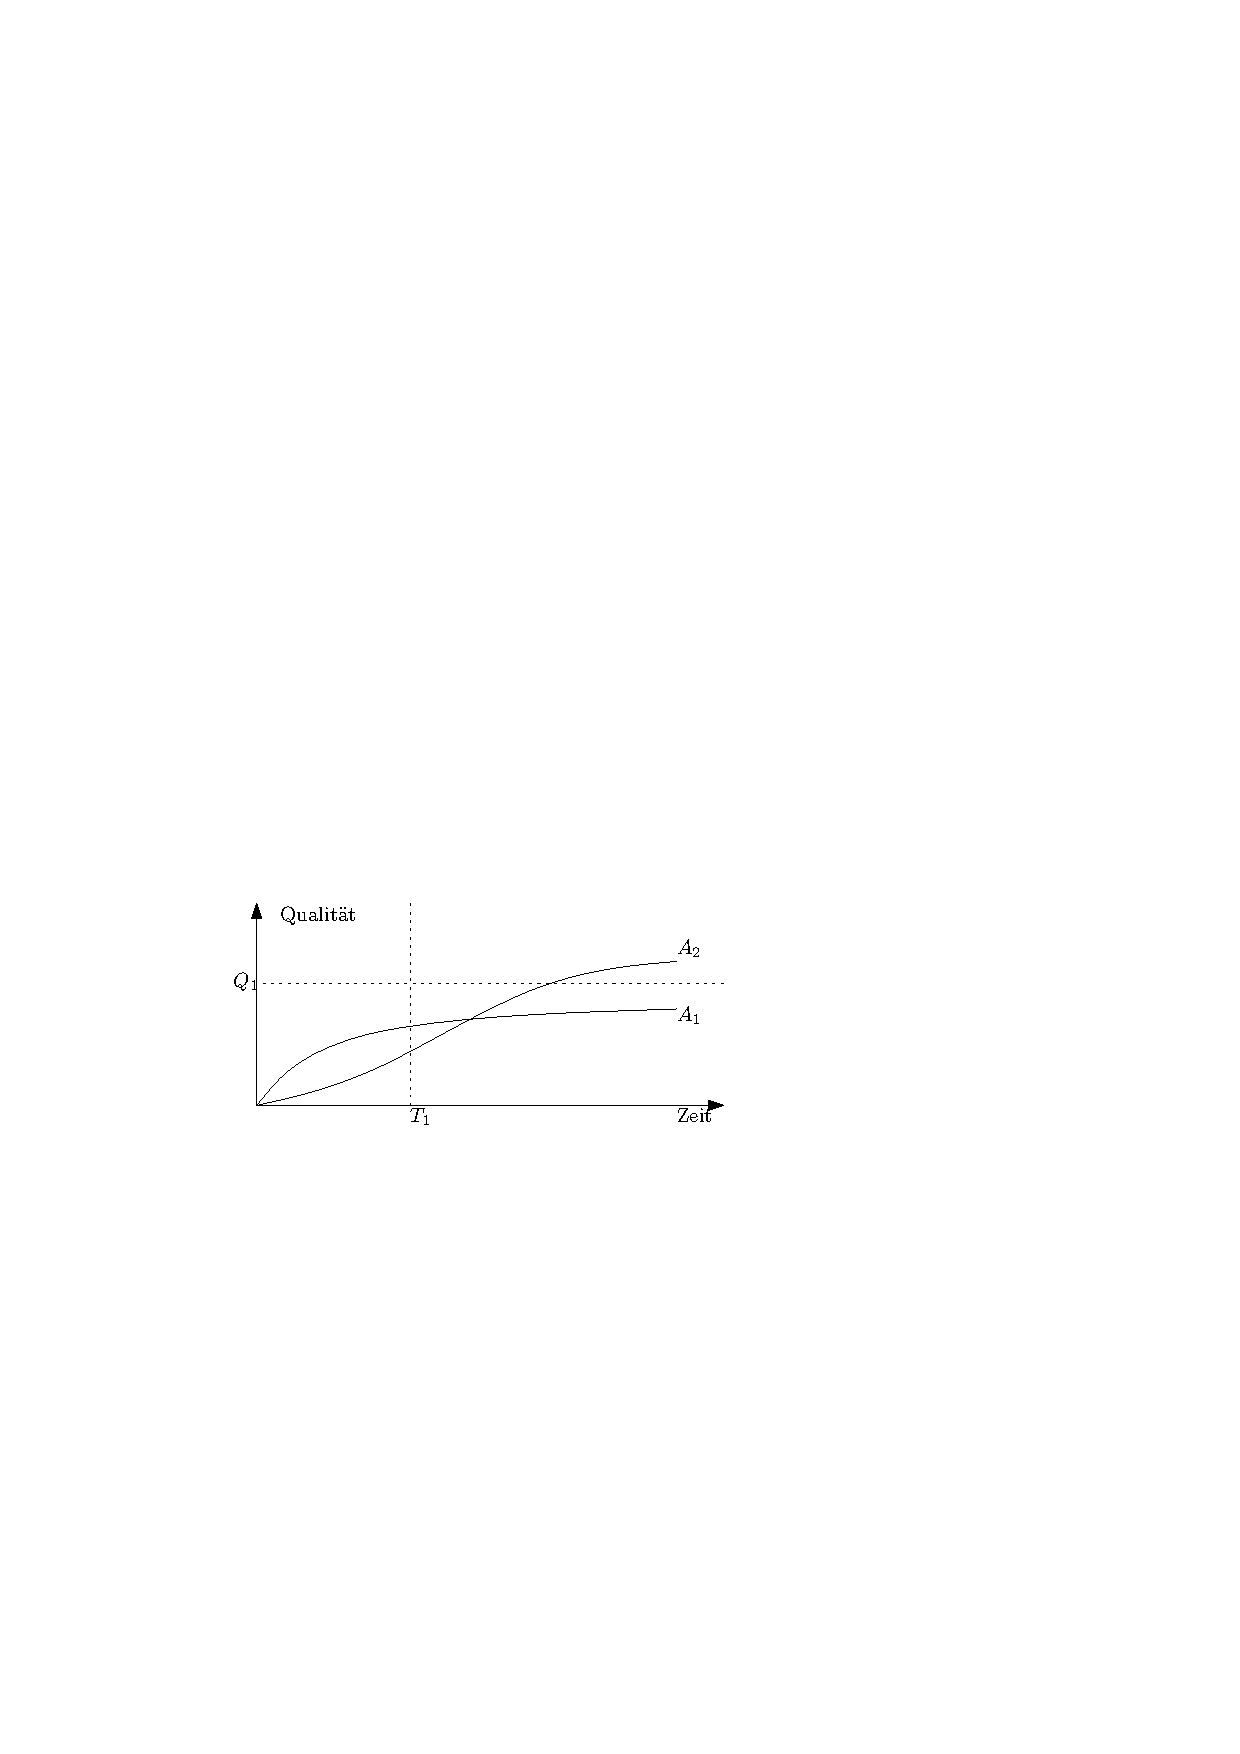
\includegraphics{timevsoptimum.pdf}
\caption[Optimierungsproblem]{Je nachdem wie die Leistung eines Algorithmus bewertet wird ändert sich der zu wählende Algorithmus. Wenn die Algorithmen beispielsweise nur $T_1$ Zeiteinheiten laufen wäre $A_1$ die beste Wahl. Die Qualitätsgrenze $Q_1$ würde jedoch $A_2$ eher erreichen.}
\label{optimizationproblem}
\end{figure}

\begin{figure}[h]
\centering
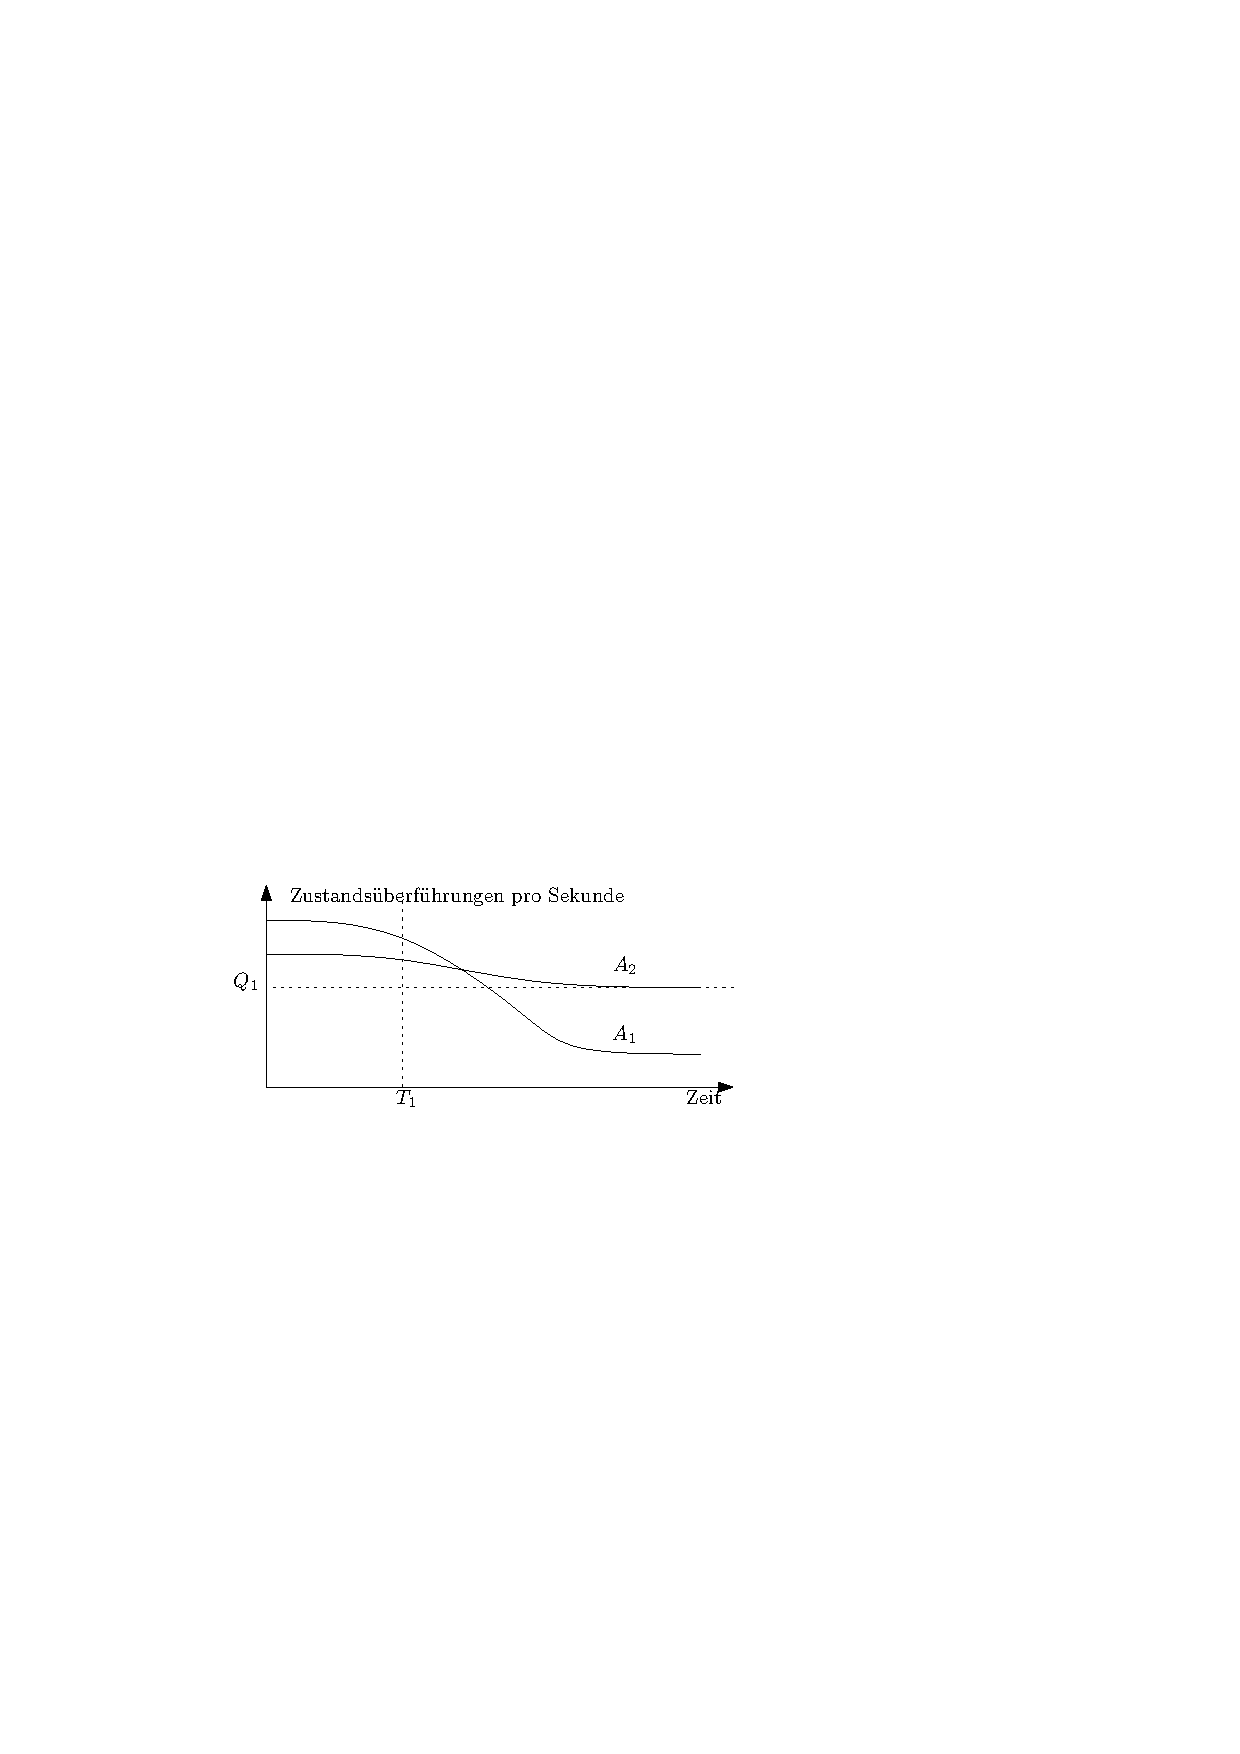
\includegraphics{ca.pdf}
\caption[Zelluläre Automaten und Algorithmenperformance]{Angenommen das Startfeld eines diskret ereignisorientierten zellulären Automaten ist hauptsächlich homogen und die Anzahl der Zellenänderungen nimmt mit jedem Zustandsübergang zu. $A_1$ könnte ein Algorithmus sein der auf wenig Zellenänderungen in einem großen Automaten spezialisiert ist. Nimmt nun die Anzahl der Zellenänderungen zu sinkt die Performance. $A_2$ hätte eine konstantere Leistung beispielsweise durch komplexe Datenstrukturen. Berechnet man nun für $T_1$ Zeiteinheiten den Automaten ist Algorithmus $A_1$ die bessere Wahl, ohne Zeitbegrenzung ist es allerdings $A_2$. Interessant wäre auch der Fall, wenn der Automat mit der Zeit wieder einen homogenen Zustand erreicht und dann wieder $A_1$ die bessere Performance aufweist. Das würde die Auswahl weiter verkomplizieren.}
\label{ca}
\end{figure}

\subsection{Kooperation von Algorithmen}

Obwohl bereits in einer der ersten Arbeiten über Algorithmenportfolios Leistungsverbesserungen durch Kooperation von Algorithmen beschrieben wurden \cite{huberman97}, wird in vielen Artikel lediglich der sogenannte Blackboxansatz verfolgt \cite{gaglioloschmidhuber06, fukunaga99, gomesselman97}. Bei diesem wird die konkrete Implementierung der Algorithmen im Portfolio nicht näher betrachtet und eine Kommunikation zwischen ihnen erfolgt nicht. Der Vorteil dabei ist, dass die Strategien für diese Portfolios auf neue Algorithmen übertragen werden können und keine Anpassungen bei neuen Problemklassen vorgenommen werden müssen. Der Nachteil ist jedoch der Verlust der Möglichkeit, Wissen zwischen Algorithmen auszutauschen und Lösungsstrukturen auszunutzen. Grundlegendes Problem beim Austausch von Wissen zwischen Algorithmen ist die meist unterschiedliche Darstellung von Zwischenergebnissen, sodass Transformationen dieser Ergebnisse durchgeführt werden müssten um sie für andere Algorithmen nutzbar zu machen. Dabei kann nicht garantiert werden, dass so eine Transformation überhaupt möglich ist und zudem sind solche Transformationen oft mit einem hohen Aufwand verbunden \cite{roberts06}. Auf der einen Seite viel menschlicher Aufwand in der Erforschung möglicher Transformationen und zum anderen ein hoher Berechnungsaufwand. Eine weitere Frage ist, wie unterschiedliche Zwischenergebnisse von Algorithmen kombiniert werden können. Bei SAT beispielsweise kann eine Formel mehrere Lösungen besitzen, welche sich gegenseitig ausschließen. Haben zwei Algorithmen nun jeweils eine andere dieser Lösungen zum Teil konstruiert, können Zwischenergebnisse beider Algorithmen gegenseitig nicht genutzt werden.

Die genannten Probleme treten im allgemeinen auch bei Simulationsalgorithmen auf. Für zelluläre Automaten existieren mehrere Darstellungsformen. Zum Beispiel Zellen als Objekte oder Zustände oder den ganzen Automaten als Bild darzustellen. Aufgrund einer wahrscheinlich sehr großen Anzahl an Zellen könnten Umformungen zwischen diesen Repräsentationen viel Zeit in Anspruch nehmen. Bei gleicher Datenrepräsentation wäre eine Anwendung von Kooperationsverfahren zweckmäßiger. Eine Bewertung solcher Verfahren wäre in dem Fall durchaus von Interesse.

\section{Ausführungsarten}

Dieser Abschnitt beschäftigt sich mit der Art der Ausführung der Algorithmen innerhalb eines Portfolios. Es werden dabei drei Typen unterschieden. Die parallele, die verschränkte und die einzelne Ausführung.

\subsection{Parallele Ausführung}

Bei der parallelen Ausführung werden die Algorithmen des Portfolios echt parallel auf mehreren Recheneinheiten ausgeführt (siehe Abbildung \ref{parallel}). Beispielsweise Gomes und Selman \cite{gomesselman97} verfolgen diesen Ansatz in Kombination mit einer Restartstrategie. Durch die parallele Ausführung müssen vorhandene Ressourcen einer Recheneinheit nicht geteilt werden, sodass der schnellste Algorithmus ohne Behinderung seine Leistung voll einbringen und ein gutes Ergebnis erzielen kann. Dazu werden natürlich genug Recheneinheiten benötigt. Des weiteren können unnötig laufende Algorithmen keine Ressourcen abgeben, sodass viele Algorithmen trotz einer erwarteten schlechten Laufzeit entweder umsonst weiter ausgeführt werden oder die entsprechenden Recheneinheiten durch einen sinnvollen Abbruch untätig sind.

Parallelität spielt bei Simulationen eine große Rolle \cite{ewald10, himmelspach09}. Modelle werden geteilt um sie parallel bearbeiten zu können. Replikationen werden parallel ausgeführt. Es gibt viele weitere Möglichkeiten allerlei Berechnungen zu parallelisieren. Die Frage dabei ist, ob eine weitere Parallelisierung bezüglich eines Algorithmenportfolios noch zweckmäßig wäre. Des Weiteren müssten langsame Algorithmen bei Simulationen, in denen jeder Verlauf in die Endergebnisse mit einfließen muss, weiter ausgeführt werden. Dann ist das Portfolio jedoch nichts anderes als eine Parallelisierung mehrerer Ausführungen einer Replikation, sofern das Portfolio nicht geändert wird. Eine Möglichkeit das zu tun wäre es beispielsweise langsame Algorithmen nach einer Durchführung aus dem Portfolio zu entfernen \cite{ewald10}. \\

\begin{figure}[h]
\centering
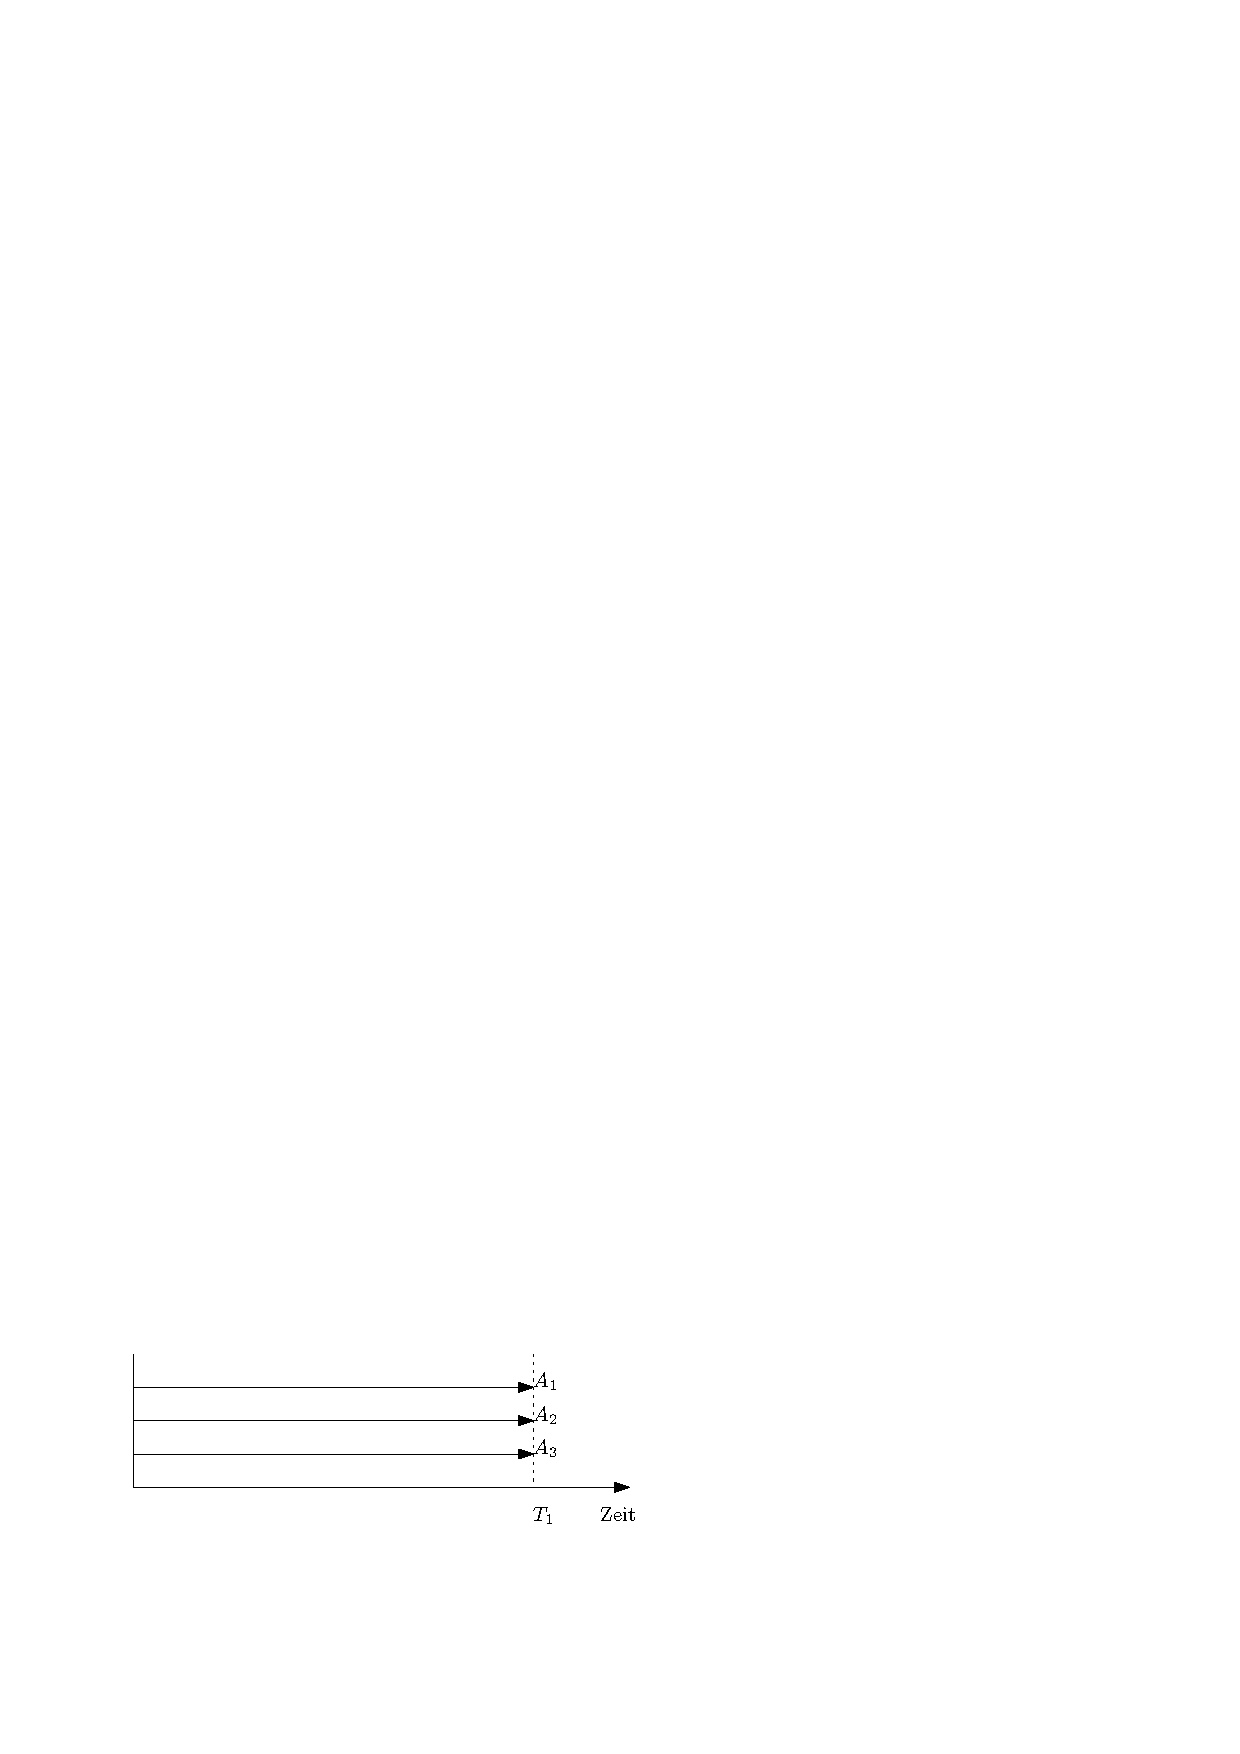
\includegraphics{parallel.pdf}
\caption[Parallele Ausf\"uhrung]{Die Algorithmen des Portfolios werden lediglich parallel ausgeführt und sobald einer von ihnen terminiert werden alle beendet.}
\label{parallel}
\end{figure}

\subsection{Verschränkte Ausführung}

Um mit einer einzelnen Recheneinheit mehrere Algorithmen parallel auszuführen wird die verschränkte Ausführung benutzt \cite{gaglioloschmidhuber06}. Die Algorithmen werden nicht echt parallel, sondern abwechselnd innerhalb eines konstanten Zeitraums ausgeführt (siehe Abbildung \ref{verschraenkt}). Dieser Vorgang wiederholt sich dann solange bis ein Algorithmus terminiert oder ein anderes Terminierungskriterium erfüllt ist. Dabei gibt es mehrere Faktoren zu beachten. Zum einen die Dauer einer Durchführung aller Algorithmen und zum anderen die Verteilung dieser Zeit auf die einzelnen Algorithmen. Verschiedene Möglichkeiten die Ressourcenverteilung anzupassen werden im Kapitel über die Entwicklung von Algorithmenportfolios näher betrachtet. Interessant ist die Tatsache, dass sich diese Art der Ausführung auch parallel mit mehreren Recheneinheiten lohnt \cite{gagliolo08}.

Bezüglich Simulationsalgorithmen ist diese Variante interessant zu Betrachten. Zum einen benötigt sie nur eine Recheneinheit und teilt sich Ressourcen selbst ein. Sollten weitere Recheneinheiten zur Verfügung stehen können sie ohne Probleme mit genutzt werden, notwendig sind sie aber nicht. Zum anderen benötigt die verschränkte Ausführung kein umfassendes Wissens über die Laufzeitverteilungen der einzelnen Algorithmen. Auch ohne dieses Wissen können gute Ergebnisse erzielt werden. \\

\begin{figure}[h]
\centering
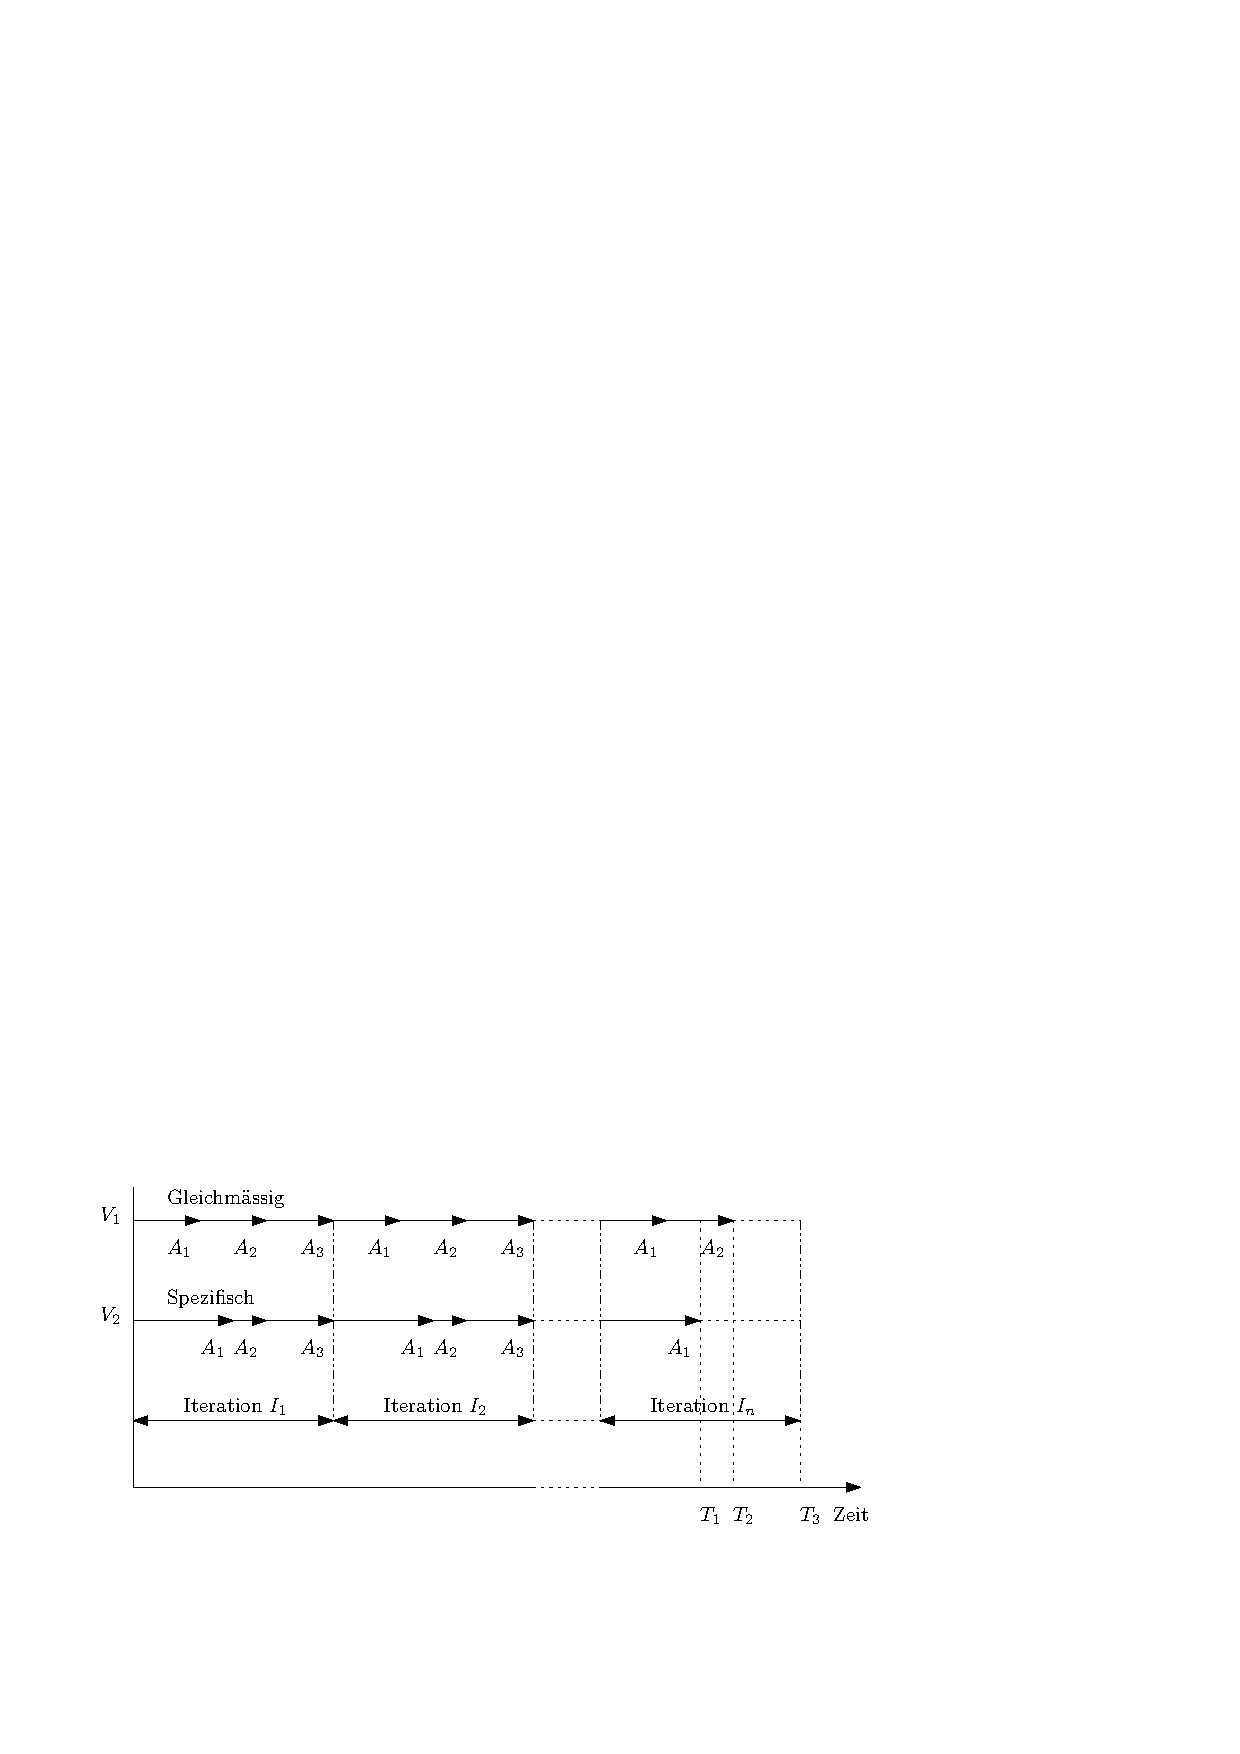
\includegraphics{verschraenkt.pdf}
\caption[Verschr\"ankte Ausf\"uhrung]{Veranschaulichung der verschränkten Ausführung eines Portfolios mit drei Algorithmen. Innerhalb einer Iteration werden alle Algorithmen einen bestimmten Anteil lang ausgeführt. Bei der Gleichbehandlung (Verlauf $V_1$) der Algorithmen terminiert $A_2$ nach n Iterationen und die Ausführung wird beendet. Wird $A_1$ jedoch bevorzugt (Verlauf $V_2$) terminiert dieser zuerst nach n Iterationen. Obwohl diese Variante schneller ist, wäre es besser $A_2$ mehr Ressourcen zur Verfügung zu stellen, da noch bessere Ergebnisse erzielt werden könnten.}
\label{verschraenkt}
\end{figure}

\subsection{Einzelne Ausführung}

Die einzelne Ausführung ist im wesentlichen nichts anderes als das ASP angewendet auf das Portfolio (siehe Abbildung \ref{einzelne}). Es wird ein Algorithmus anhand erstellter Leistungsdaten für eine Probleminstanz ausgewählt und nur dieser wird dann zur Problemlösung ausgeführt. Der Vorteil gegenüber dem allgemeinen ASP ist die kleinere Menge an Algorithmen im Portfolio. Zusätzlich ist eine Wettbewerbsphase möglich. In dieser werden alle Algorithmen ähnlich wie bei der verschränkten Ausführung bis zu einem bestimmten Zeitpunkt ausgeführt. Die aktuelle Leistung der Algorithmen wird dann verglichen und der beste wird zur alleinigen Ausführung ausgewählt. Die nach \cite{roberts06} am meisten verwendeten Faktoren zur Berechnung der Leistung sind das aktuelle Zwischenergebnis, bei Simulationen beispielsweise der aktuelle Zustand eines zellulären Automaten, die vorhergesagte Restlaufzeit und die bisherige Auswahlrate des Algorithmus.

Es ist naheliegend, dass dieser Ansatz mit genügend Leistungsdaten der Effektivste ist. Jedoch sind genau diese Leistungsdaten meistens nicht vorhanden. Das ist auch bei Simulationsalgorithmen nicht anders. Ein Vorteil dieser Ausführung ist, dass jeder Lauf bis zum Ende ausgeführt wird und in der Ergebnisanalyse berücksichtigt werden kann. \\


\begin{figure}[h]
\centering
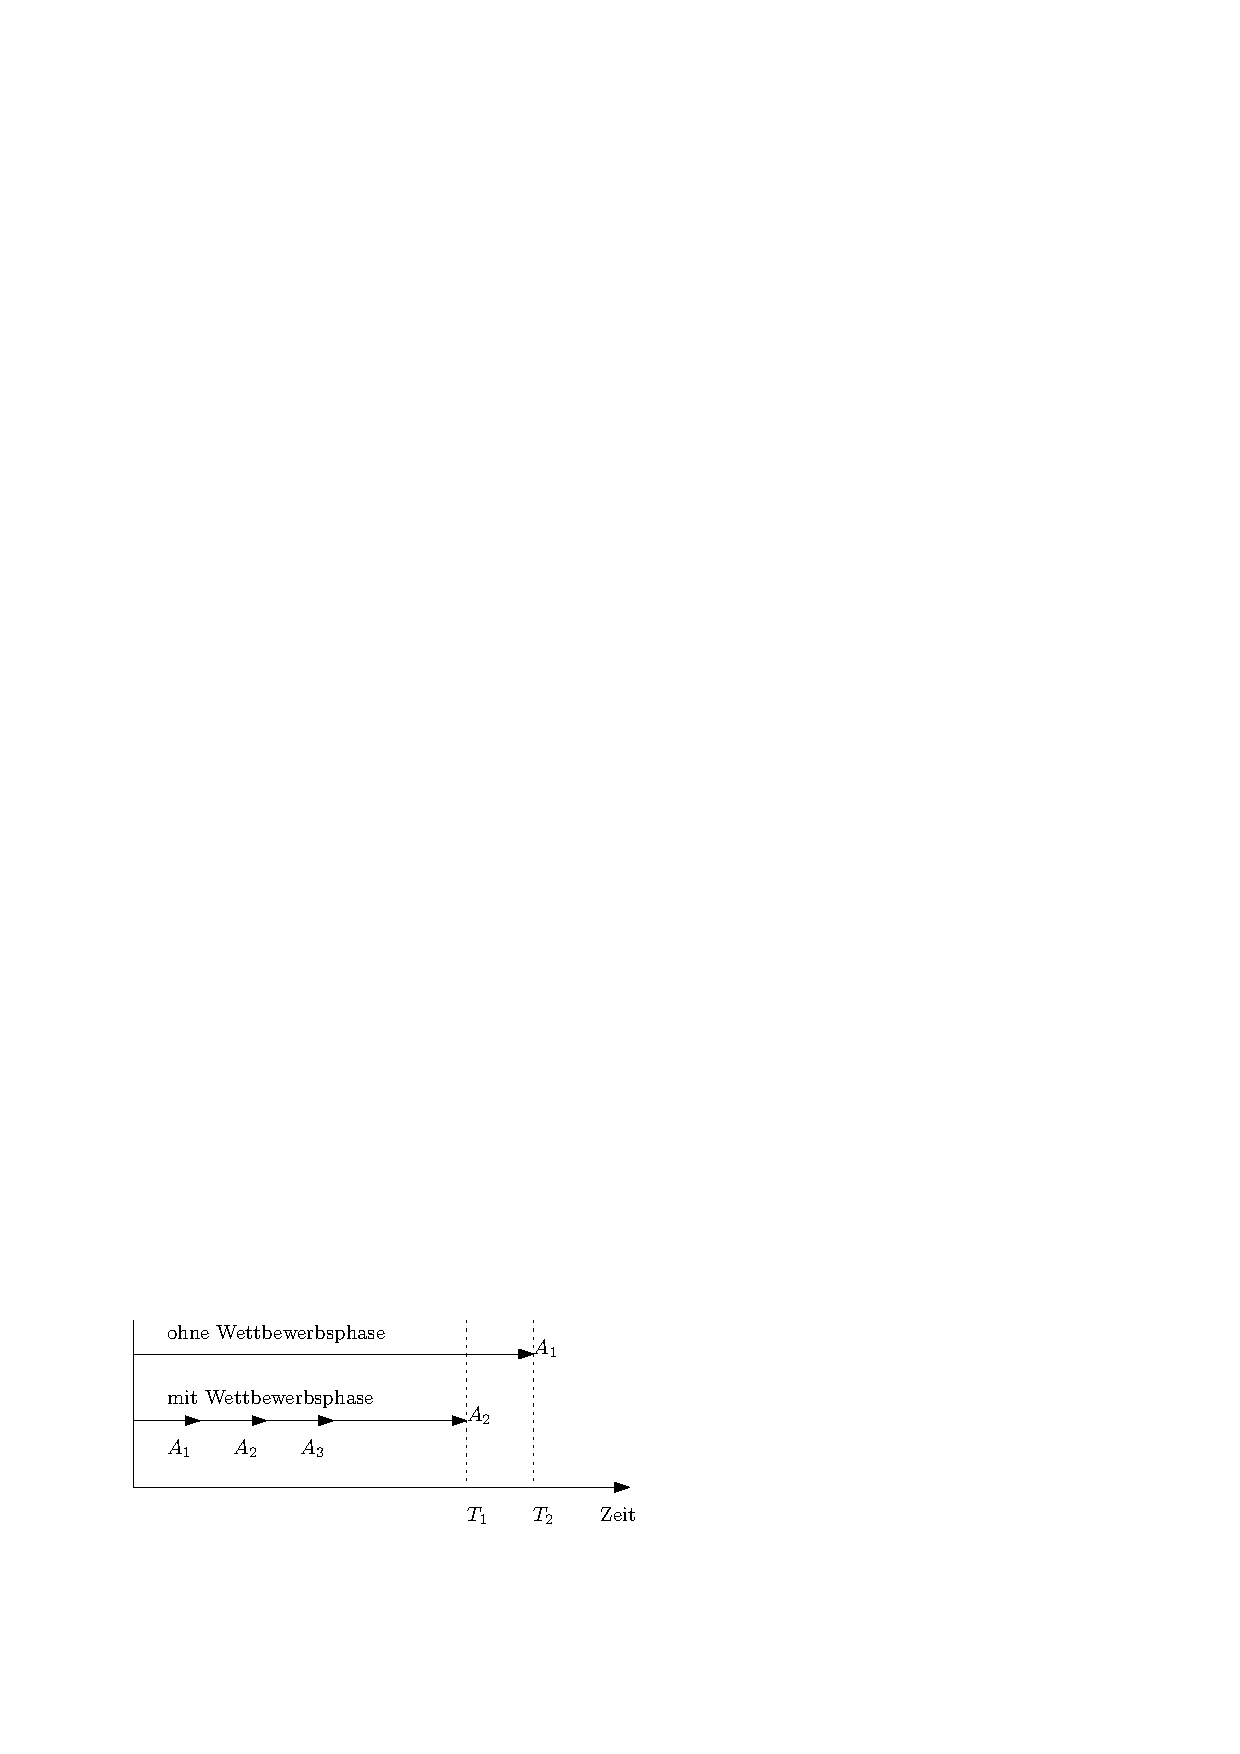
\includegraphics{einzelne.pdf}
\caption[Einzelne Ausf\"uhrung]{Beispiel für die einzelne Ausführung eines Portfolios mit drei Algorithmen. Ohne Wettbewerbsphase wird direkt ein Algorithmus für die Problemlösung ausgewählt, in dem Fall $A_1$. Nach einer Wettbewerbsphase der drei vorhandenen Algorithmen würde jedoch $A_2$ als der erfolgversprechendere Kandidat erkannt. Dieser ist dann so performant, dass trotz Wettbewerbsphase ein besseres Ergebnis als bei der alleinigen Ausführung von $A_1$ erreicht wird.}
\label{einzelne}
\end{figure}

\section{Entwicklung eines Algorithmenportfolios}

Bei der Entwicklung von Portfolios geht es hauptsächlich um eine Neuverteilung der ver"-fügbaren Ressourcen während der Konstruktion und Benutzung eines Portfolios (siehe Abbildung \ref{entwicklung}). Grundsätzlich muss zwischen der Entwicklung des Portfolios an sich und der Entwicklung der einzelnen Algorithmen unterschieden werden. Auf die Entwicklung von Algorithmen soll an dieser Stelle nicht näher eingegangen werden. Es sei lediglich erwähnt, dass lernfähige Algorithmen zusätzliche Redundanzen in der Datenbasis schaffen könnten und dann eine unnötige Belastung für das Portfolio erzeugen \cite{roberts06}. Zudem muss bei einem Portfolio mit lernfähigen Algorithmen immer darauf geachtet werden, dass mit einer zunehmenden Anzahl von Problemlösungen eine Erhöhung der Leistung nicht nur durch eine Verbesserung des Portfolios, sondern auch durch die verbesserten Algorithmen zustande kommt.

Vor allem die verschränkte Ausführung von Algorithmen findet bei der Analyse der Entwicklungsstrategien große Beachtung. Parallele Portfolios können eine Verteilung der verfügbaren Ressourcen nicht ändern und Auswahlportfolios können auf die Theorie des ASP und in der Wettbewerbsphase auf die Ergebnisse der verschränkten Portfolios zurückgreifen.

Die Entwicklung von Algorithmenportfolios lässt sich grob in zwei Phasen unterteilen. Zum einen in eine Trainingsphase, in der Lösungen für repräsentative Probleminstanzen $R_1, ..., R_n$ berechnet werden. Sowohl repräsentative Probleminstanzen für die Trainings"-phase, als auch eine optimale Anzahl jener zu finden sind schwierige Aufgaben \cite{gaglioloschmidhuber06}. Mithilfe der Ergebnisse der Trainingsphase wird eine Datenbasis erstellt, welche für die zweite Phase, die Ausführungsphase genutzt wird. In dieser werden Lösungen für alle weiteren auftretenden Probleme berechnet. 

Die besten Ergebnisse werden bei der Entwicklung von Portfolios erzielt, in denen jeweils ein dominierender Algorithmus für eine Probleminstanz existiert \cite{gomesselman97, gaglioloschmidhuber06}. Diese werden ab einem bestimmten Punkt den Großteil der Ressourcen zur Verfügung haben. Existieren mehrere ähnliche Algorithmen werden sich die Ressourcen ungünstigerweise gleichmäßig unter ihnen aufteilen.

\begin{figure}[h]
\centering
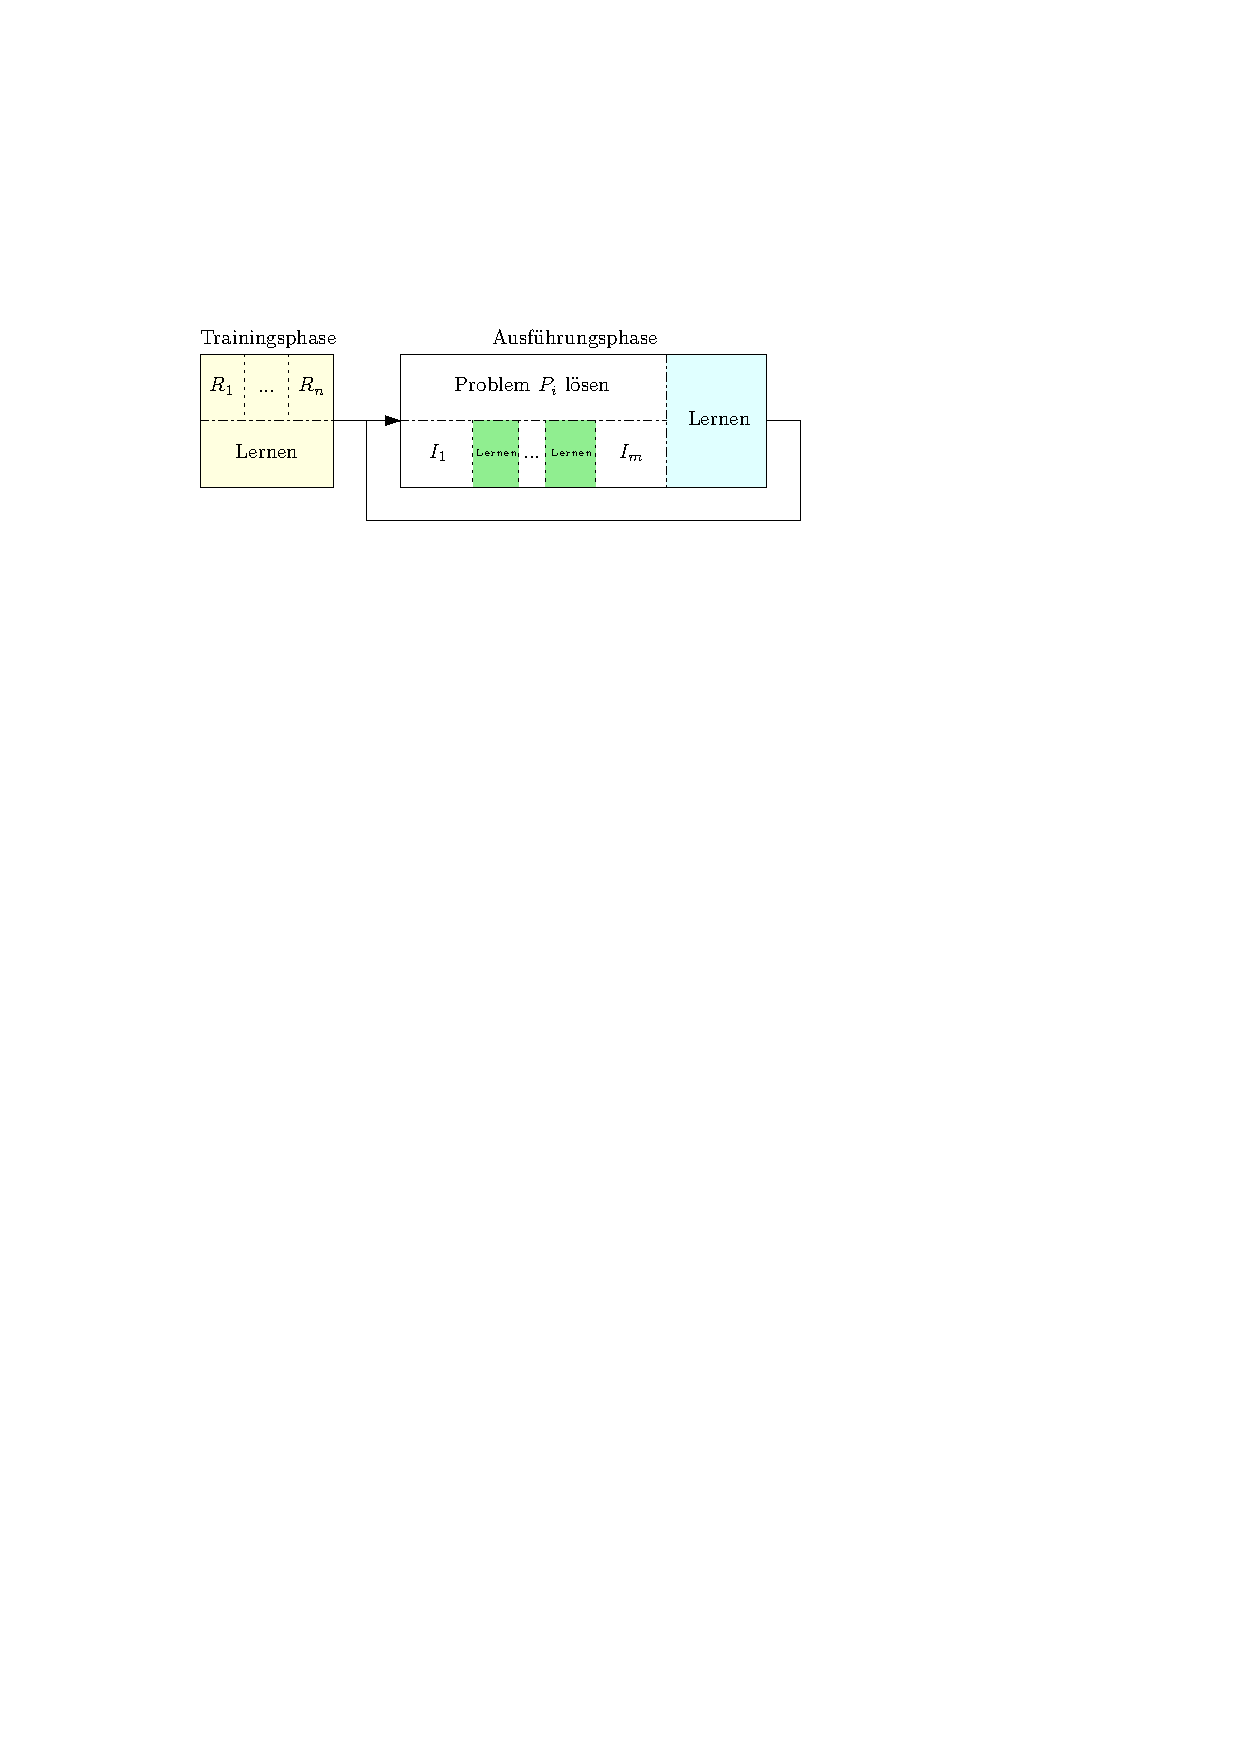
\includegraphics[scale=1.3]{progress.pdf}
\caption[Entwicklung eines Algorithmenportfolios]{Überblick über die Entwicklungsarten eines Portfolios. In der Trainingsphase (gelb) werden $n$ repräsentative Probleme $R_1$ bis $R_n$ gelöst und eine Datenbasis wird anhand der Ergebnisse erstellt. Diese Datenbasis wird in der Ausführungsphase eingesetzt und bei einer Offlineentwicklung (blau) nach jeder Problemlösung durch weiteres Lernen verbessert. Bei der Onlineentwicklung (grün) wird zusätzlich zwischen jeder Iteration innerhalb einer Problemlösung die Datenbasis für dieses jeweilige Problem angepasst.}
\label{entwicklung}
\end{figure}

\subsection{Statische Entwicklung}

Die statische oder vergessliche \cite{gaglioloschmidhuber06} Entwicklung hält sich an die klare Trennung von Trainings- und Ausführungsphase. Es wird zwischen der Berechnung einzelner Probleminstanzen keine Veränderung der Strategie des Portfolios vorgenommen. Ein Nachteil dabei ist, dass die Trainingsphase viele Probleme umfassen muss um gute Ergebnisse zu liefern und dennoch wird das System unflexibel gegenüber neuartigen Problemen sein. Ein Lösungsansatz zur Vermeidung solch einer umfangreichen Trainingsphase ist es Ungenauigkeiten in der Datenbasis zu akzeptieren. Beispielsweise indem langsame Algorithmen nach einer bestimmten Laufzeit oder einer bestimmten Quote von beendeten Algorithmen abgebrochen werden \cite{gaglioloschmidhuber06}. Dadurch werden unnötig lange Berechnungszeiten vermieden.

Die daraus resultierende Ungenauigkeit hat keine größeren Auswirkungen auf die Ergebnisse des gesamten Portfolios, da sehr langsame Algorithmen sowieso nicht bis zur Beendigung ausgeführt werden, sodass diese Methode gute Ergebnisse erwarten lässt. Das einzige Problem ist es einen guten Zeitpunkt für den Abbruch zu finden.

Für Simulationsalgorithmen ist der Einsatz dieser Art der Entwicklung wahrscheinlich nicht zweckmäßig. Ein Simulationslauf kann viele Iterationen ähnlicher Berechnungen haben, sodass sich die negativen Auswirkungen einer ungünstigen Ressourcenverteilung vielfach addieren würden \cite{ewald10}.

\subsection{Dynamische Entwicklung}
\label{dynamisch}

Neben der klaren Trennung zwischen Trainings- und Ausführungsphase gibt es dynamische Ausführungsphasen, in denen sich die Strategie des Portfolios verändern kann. Es werden zwei Typen unterschieden, die Offline- und die Onlineentwicklung. 

Im Zusammenhang mit Simulationsalgorithmen kann keine der beiden Varianten generell favorisiert werden. Je nach Anwendung kann die eine oder die andere Methode besser sein. Würde man beispielsweise als Probleminstanz die Berechnung von 1000 Zustandsübergängen eines zellulären Automaten heranziehen, könnte eine Verteilung der Res"-sourcen zu Beginn der Berechnungen nicht optimal sein. Eine Anpassung innerhalb der Berechnungen wäre zweckmäßig. Würden jedoch viele solcher Replikationen berechnet werden, könnte eine Offlineentwicklung möglicherweise nach einigen Problemen schon eine gute Verteilung der Ressourcen liefern, sodass die Onlineentwicklung nur wenig Anpassung durchführen würde, welche den zusätzlichen Aufwand nicht rechtfertigt.

\subsubsection*{Offline}

Bei der Offlinemethode werden Messdaten einer durchgeführten Berechnung in der Aus"-führungsphase genutzt um die vorhandene Strategie zu verbessern. Die Verteilung von Ressourcen an Algorithmen kann sich somit zwischen dem Lösen von Probleminstanzen ändern. Diese Maßnahme erhöht die Flexibilität des Portfolios gegenüber neuen Problemarten, welche in der Trainingsphase unberücksichtigt waren. In Folge der immer neu erhaltenden Daten kann die Trainingsphase verkürzt werden. Damit einseitige Probleminstanzen zu Beginn der Ausführungsphase das Portfolio nicht zu stark in eine Richtung spezialisieren sollte der Grad der Berücksichtigung neuer Ergebnisse zu Beginn niedrig sein und nur langsam ansteigen \cite{gaglioloschmidhuber06}.

\subsubsection*{Online}

Die Onlinemethode geht noch einen Schritt weiter und aktualisiert die Ressourcenverteilung des Portfolios während einer Problemlösung. In \cite{gaglioloschmidhuber06} wird dieser Ansatz verfolgt und ausführlich analysiert. Nach einer Iteration aller beteiligten Algorithmen werden die aktuellen Zwischenergebnisse oder die Vorhersagen über die zu erwartende Restlaufzeit oder weitere Kriterien benutzt um die Ressourcen neu aufzuteilen. Auf der einen Seite kann konkret auf Probleminstanzen individuell reagiert werden. Auf der anderen Seite jedoch werden starke Startalgorithmen womöglich gegenüber im Endergebnis besseren Algorithmen bevorzugt. In Folge dessen kann die Gesamtleistung des Systems schlechter sein als bei einer gleichmäßigen Ressourcenverteilung (siehe Abbildung \ref{online}). Um solchen Fehlentwicklungen entgegenzuwirken muss genau wie bei der Offlineentwicklung der Grad der Berücksichtigung aktueller Ergebnisse am Anfang niedrig sein und langsam ansteigen. \\


\begin{figure}[h]
\centering
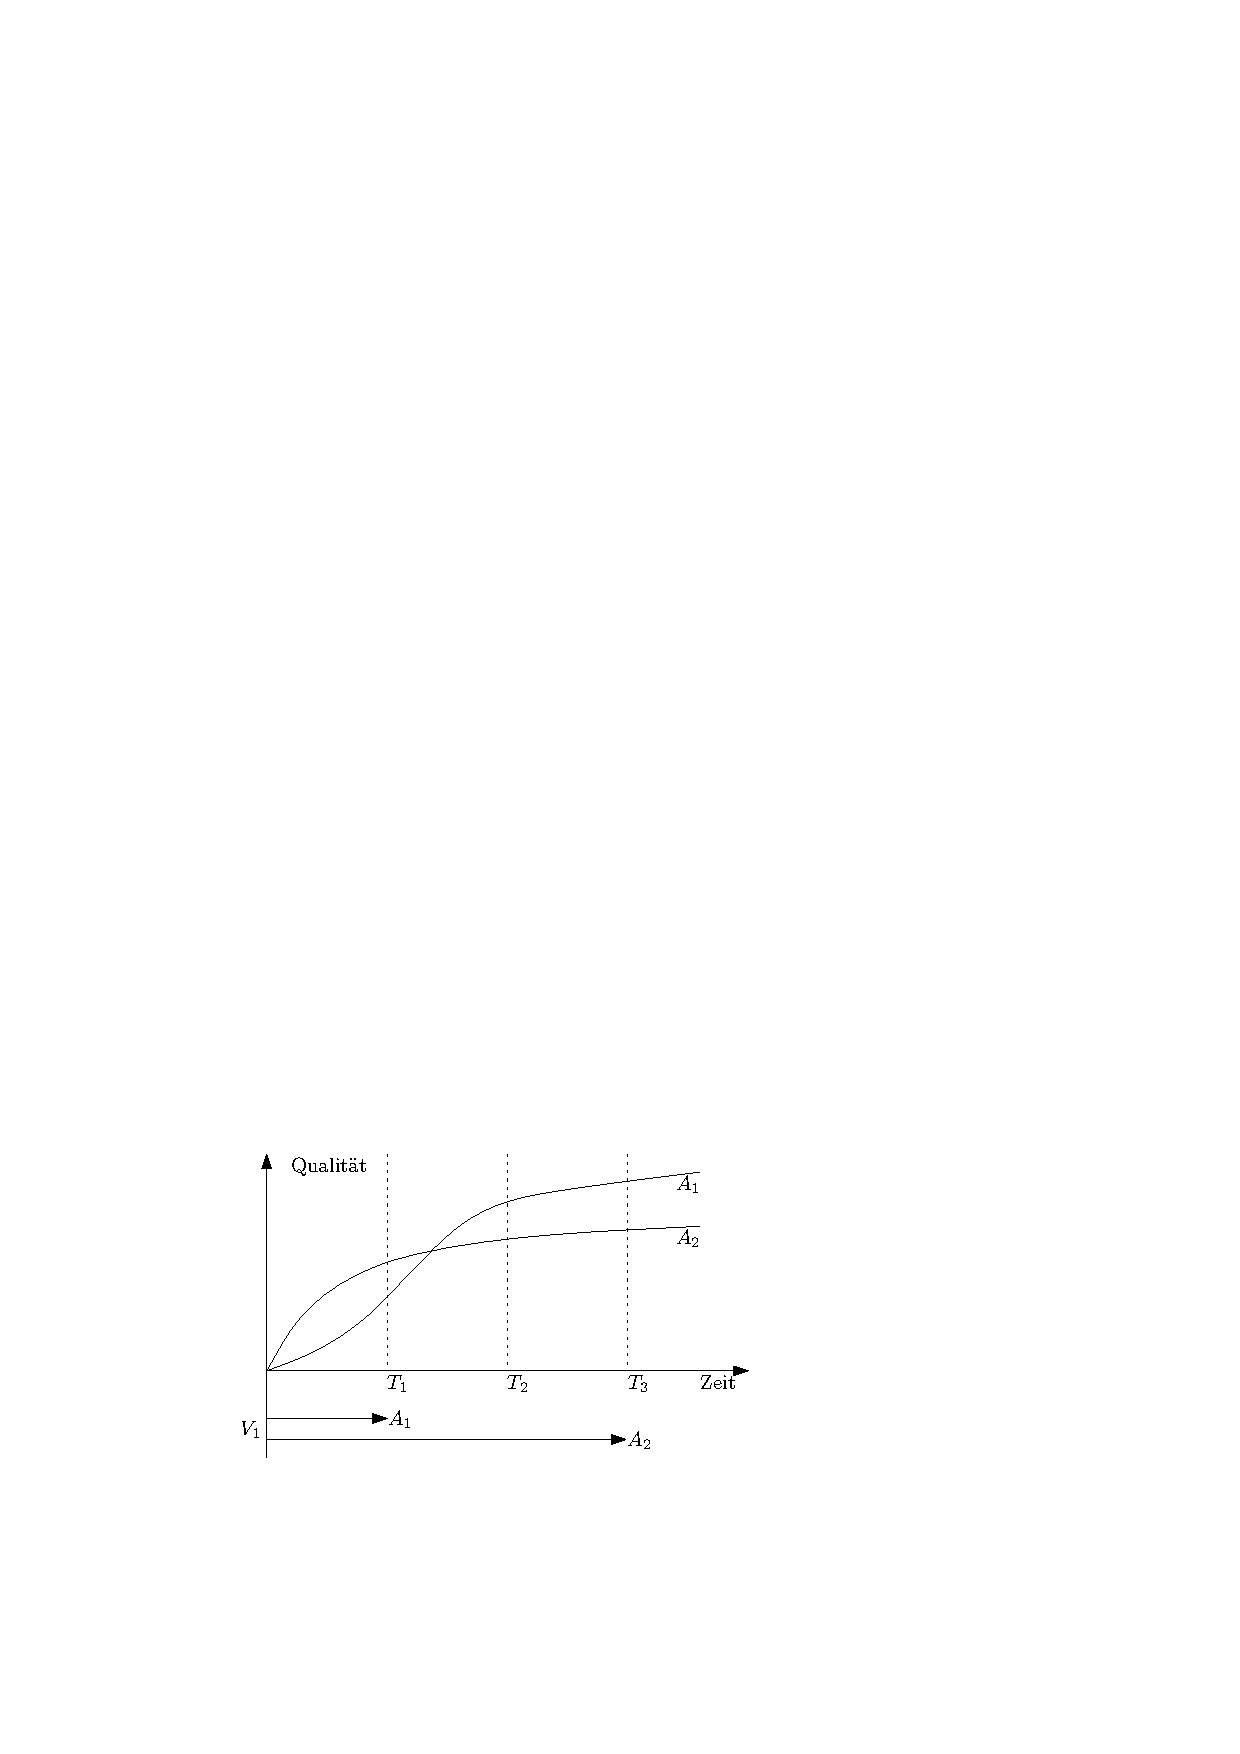
\includegraphics{onlineproblem.pdf}
\caption[Onlineentwicklungsproblem]{Veranschaulichung des grundlegenden Problems der Onlineentwicklung. $2 \cdot T_2$ Zeiteinheiten stehen zur Verfügung und sie werden aufgrund der guten Anfangsergebnisse von $A_2$ entsprechend des Verlaufs $V_1$ verteilt. $A_2$ läuft bis $T_3$ und $A_1$ bis $T_1$. Das Ergebnis ist dadurch sogar schlechter, als würden beide Algorithmen gleichberechtigt $T_2$ Zeiteinheiten ausgeführt.}
\label{online}
\end{figure}



